\begin{wrapfigure}[13]{r}{0.5\linewidth}
\centering
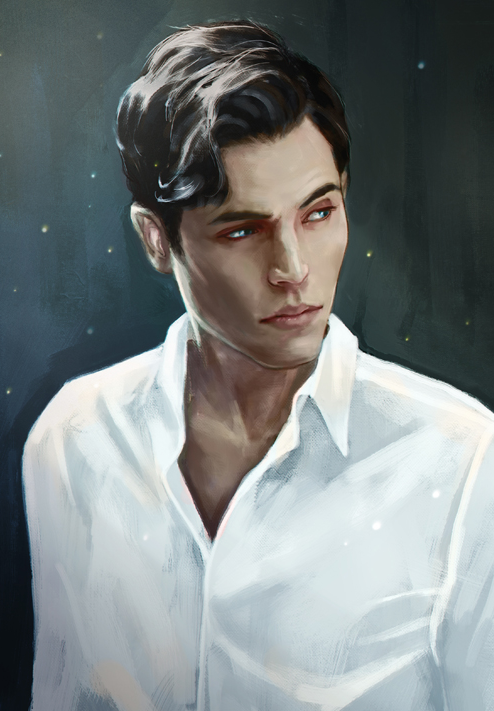
\includegraphics[max width=0.5\textwidth]{../Pictures/Characters/Portraits/Tom_portrait.png}
\end{wrapfigure}

\paragraph{Description}
Tom Marvolo Riddle is a black-haired half-blood wizard. He is currently a model student at Hogwarts where he was sorted into the Slytherin House, a nod to his ancestor Salazar Slytherin; there he gained the sympathy of many amongst the school's staff and students thanks to his particular charisma and oratory abilities, notably professor Slughorn. 

The sole exception to this was Dumbledore, who never forgot about his misdeeds at the orphanage, nor his unsettling behaviour during their first meeting: this made Tom realize his mistake of showing too much of his real self to Dumbledore, growing up to fear and despise him, unable to manipulate him anymore.

\paragraph{Backstory}
Tom Riddle was born in an orphanage in London, where his mother died shortly after giving birth to him. He grew up completely unaware of his wizarding heritage until he discovered that he could make things move without touching them, speak to snakes and... "make bad things happen to mean people". He finally understood the meaning of that after the meeting with Dumbledore, which convinced him to deepen his knowledge at Hogwarts, albeit feeling hindered by the rules.

\begin{figure}[H]
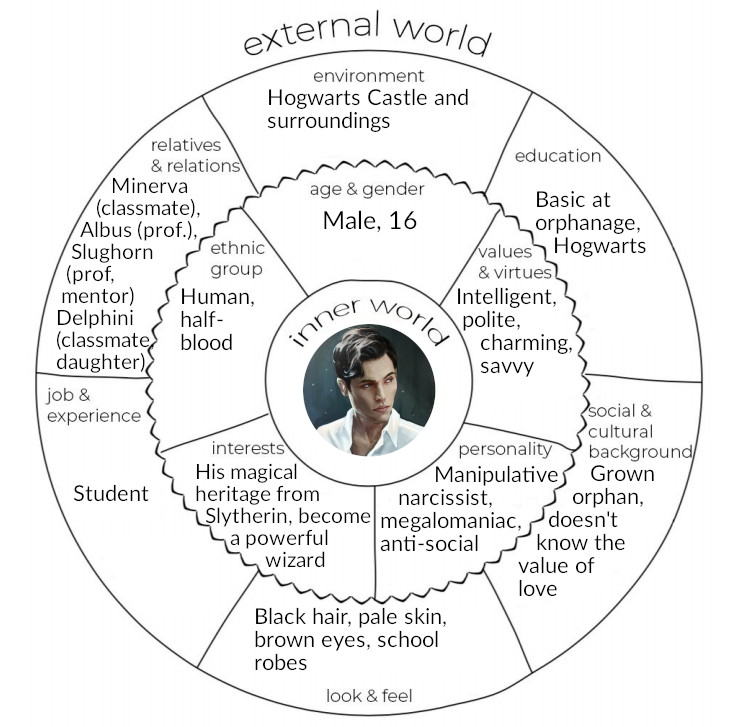
\includegraphics[max width=\textwidth]{../Pictures/Characters/Circumplexes/Tom_circumplex.png} 
\captionsetup{labelformat=empty}
\caption{Circumplex}
\end{figure}

\begin{figure}[H]
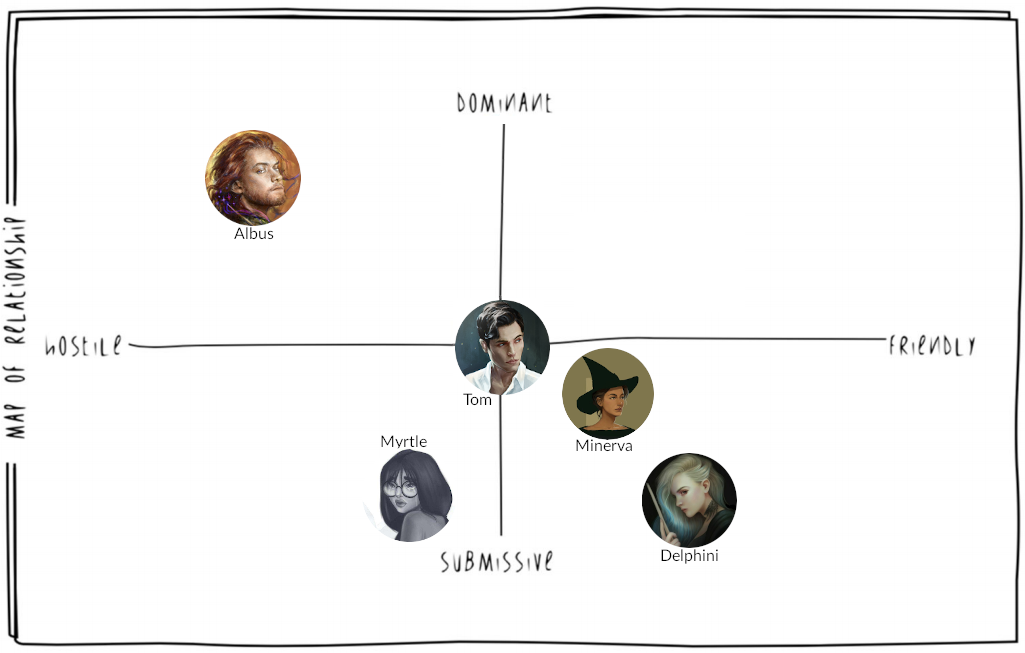
\includegraphics[max width=\textwidth]{../Pictures/Characters/Relationship_maps/Tom_relmap.png} 
\captionsetup{labelformat=empty}
\caption{Map of relationships}
\end{figure}


\clearpage